\documentclass[11pt]{report}
\usepackage{graphicx}
\usepackage{amssymb}
\usepackage{amsthm}
\usepackage{fullpage}
\usepackage{tikz}
\tikzset{node distance=2cm, auto}
\DeclareGraphicsRule{.tif}{png}{.png}{`convert #1 `dirname #1`/`basename #1 .tif`.png}

%%%%%%%%%%%%%%%%%%%%%%%%%%%%%%%%%%%%
%%%%%%%%%%%%%%%%%%%%%%%%%%%%%%%%%%%%
\newcommand{\Q}{\mathbb{Q}}
\newcommand{\Z}{\mathbb{Z}}
\newcommand{\C}{\mathbb{C}}
\newcommand{\R}{\mathbb{R}}
\newcommand{\N}{\mathbb{N}}
\newcommand{\M}{\mathcal{M}}
\newcommand{\Zp}{\mathbb{Z}/p\mathbb{Z}}
\newcommand{\Zn}{\mathbb{Z}/n\mathbb{Z}}
\newcommand{\Zm}{\mathbb{Z}/m\mathbb{Z}}
\newcommand{\bl}{\ & \ & \\}
\newcommand{\eql}{\ & = &}
\newcommand{\ba}{\\ \begin{array}{rcl}}
\newcommand{\ea}{\end{array} \\}
\newcommand{\claim}{\underline{Claim}: \ }
\newcommand{\pf}{\underline{Proof of Claim}: \\ }
\newcommand{\mat}{\left[\begin{array}{cc} a & b \\ c & d \end{array}\right]}
\newcommand{\lra}{\longrightarrow}
\newcommand{\mf}{\mathfrak}
\newcommand{\inv}{^{-1}}
\newcommand{\ML}{\mathcal{L}}
\newcommand{\LM}{\mathcal{L}}
\newcommand{\LMEF}{\mathcal{L}(E;F)}
\newcommand{\Mnn}{M(n\times n)}
\newcommand{\OnR}{O(n;\R)}
\newcommand{\XM}{\mathfrak{X}(M)}
\newcommand{\eps}{\epsilon}
\newcommand{\CM}{C^{\infty}(M)}
\newcommand{\ddt}{\frac{d}{dt}}
\newcommand{\dds}{\frac{d}{ds}}
\newcommand{\Zhat}{\hat{\mathbb{Z}}}
\newcommand{\coker}{\text{coker}}
\newcommand{\Hom}{\text{Hom}}
\newcommand{\End}{\text{End}}
\newcommand{\Aut}{\text{Aut}}
\newcommand{\Tr}{\text{Tr}}
\newcommand{\ra}{\rightarrow}
\newcommand{\Ra}{\Rightarrow}
\newcommand{\mfp}{\mathfrak{p}}
\newcommand{\mfq}{\mathfrak{q}}
\newcommand{\mfm}{\mathfrak{m}}
\newcommand{\Ap}{A_{\mathfrak{p}}}
\newcommand{\OK}{\mathcal{O}_k}
\newcommand{\Zx}{\mathbb{Z}[x]}
\newcommand{\Zxn}{\mathbb{Z}[x_1,\ldots,x_n]}
\newcommand{\Zxy}{\mathbb{Z}[x,y]}
\newcommand{\Zpxy}{\mathbb{Z}/p\mathbb{Z}[x,y]}
\newcommand{\beq}{\begin{equation*}}
\newcommand{\eeq}{\end{equation}}
%\setlength{\parindent}{0cm}        % \noindent everywhere!
%%%%%%%%%%%%%%%%%%%%%%%%%%%%%%%%%%%%
%%%%%%%%%%%%%%%%%%%%%%%%%%%%%%%%%%%%

\setcounter{tocdepth}{3}

\title{Homomorphic Encryption}
\author{Ben LeVeque}
\date{\today}         

\begin{document}
\maketitle


\tableofcontents

\newpage

\section[Intro]{Introduction and background}

In an age of ubiquitous computing, digital security is an important aspect of everyday life. As computations involving large data sets become more expensive and time-consuming, and as the need for data storage increases, cloud computing has rapidly developed to become a platform to which people and institutions alike turn for their computational needs. With this rise in popularity comes the need for a new class of security protocols that allow data to be stored in encrypted form yet manipulated in a meaningful way by third parties. In this thesis, we consider two such cryptographic schemes. We discuss the motivation behind them, analyze their security, and present data regarding both their security and efficiency. We also provide implementations of the systems in question in C++ and explain the code's design.

Two goals in the very close periphery throughout the development of this project have been reproducibility and accessibility. In this vein, the implementations produced and the data generated are posted in a public repository on Github at (ADDRESS), and a website accompanying the project can be found at (ADDRESS).

\subsection{Introduction to cryptographic concepts and terminology} 

INTRO SENTENCE. A \emph{message} (also called a \emph{plaintext}) is any information you might want to store securely. For example, an email or a bank statement. An \emph{encryption function} accepts this message and outputs a corresponding \emph{ciphertext}, from which it should be very difficult to 

Often, this message is first \emph{encoded} to transform it into a value which can 
Introduce idea of FHE. Define terms (plaintext, ciphertext, message, message space, ciphertext space, cryptosystem, encryption, key generation, decryption $\N=\Z_{\geq 0}$).

\

\subsection{Introduction to homomorphic encryption}

Imagine you have a large collection of data points and want to compute the mean or standard deviation. You have have two options: you can either do this computation yourself at a potentially high computational cost, or you can delegate this work to another party and risk losing privacy.  The goal of fully homomorphic encryption is to minimize both potential costs by allowing secure delegation. In practice, this might mean being able to store data on the Cloud in an encrypted form such that a third party could still manipulate the data in a meaningful way. By meaningful, we simply mean that after they operate on our data, we can decrypt the result and obtain exactly the value their operations would have achieved on our original plaintext data. The following diagram shows this process:

\

$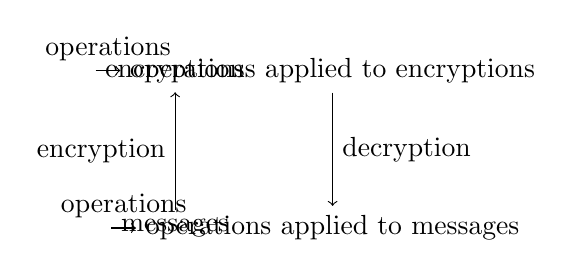
\begin{tikzpicture}
\node (m) {messages};
\node (fm) [right of=m] {operations applied to messages};
\node (em) [above of=m] {encryptions};
\node (fem) [right of=em] {operations applied to encryptions};
\draw[->] (m) to node {operations} (fm);
\draw[->] (fem) to node {decryption} (fm);
\draw[->] (m) to node {encryption} (em);
\draw[->] (em) to node {operations} (fem);
\end{tikzpicture}$

\

More technically, by ``meaningful'' we mean that any combination of sums and products of encryptions decrypt to the corresponding sums and products of the original, unencrypted data. We call such a combination an \emph{arithmetic circuit}, or just a \emph{circuit}. If this were possible, data could be encrypted, operated upon, and decrypted in a completely well-defined manner. What we are looking for, then, is an encryption function that is a \emph{ring homomorphism} from the message space $\M$ to the ciphertext space $\mathcal{C}$. Recall that a ring homomorphism is a map $\sigma: \M \rightarrow \mathcal{C}$ such that for any $x,y\in \M$, \[\sigma(x)+\sigma(y) = \sigma(x+y)\] \[\sigma(x) \sigma(y) = \sigma(xy)\] If our encryption function $e$, then, is a ring homomorphism, we could add or multiply two encryptions and the result would be the encryption of the sum or product of the corresponding plaintexts. A cryptosystem employing such an encryption function is said to give \emph{fully homomorphic encryption} (FHE). If the encryption function in question is a homomorphism in most circumstances, but is not guaranteed to give well-defined decryption after the application of every circuit, the scheme is said to provide \emph{somewhat homomorphic encryption}. Such a scheme might arise if the decryption function requires its input to be of a certain size, which large circuits might exceed. For motivation, consider the following toy examples.

\

First, we will construct a somewhat homomorphic encryption scheme that provides very little security but illustrates the concepts presented above. Consider the message space $\M = \N$ and choose as a secret key some prime number $p$. We will encrypt a message $m\in \M$ by setting $e(m) = m+ap$ for some random integer $a$. Decryption is then performed by reducing modulo $p$. As long as the message $m$ is less than $p$, this scheme is perfectly well defined, since \[d(e(m)) = m+ap \pmod{p} = m\] However, if $m\geq p$, then $d(e(m))$ will no longer equal $m$, but will be the reduction of $m$ modulo $p$. One way to attempt to avoid this problem is to encrypt values only less than $p$. However, once we start considering circuits applied to encryptions, this idea shows its flaws; the sum of two encryptions of $p-1$, for example, would really be an encryption of $2p-2$, but it would encrypt to $-2 \equiv p-2 \pmod{p}$. Another solution is to recognize the limitations of the system and include as a part of the system's protocol a bound on the number of additions and multiplications that can be performed on encryptions before the result should be decrypted. 

To make this scheme fully homomorphic, we could set $\M = \Zp$, since in this case, reducing modulo $p$ during decryption is consistent with the structure of the message space. However, it is perhaps unnatural to for messages to live in $\Zp$, since when we compute, for example, standard deviations, we don't want to reduce modulo $p$ at any point during the computation. In this case, it may be best to accept the limitations of the somewhat homomorphic scheme above and work within its framework.

It should be mentioned, as well, that the scheme above is just a ``toy'' example because it is very insecure. Suppose an eavesdropper asked us to encrypt the message $m=0$ using this system. The result would be a multiple of $p$. Suppose we were asked to perform many such encryptions. We would end up with a collection of multiples of $p$. With this information, it would be very fast to compute the greatest common divisor of these values using the Euclidean Algorithm, and the result would likely be $p$ itself. Using $p$, the eavesdropper could then decrypt any message he pleased by simply reducing it modulo $p$. This type of attack---using encryptions of the message $0$ to reveal an essential feature of the structure of the scheme itself---will appear again, and is a necessary threat to consider when formulating encryption schemes. This attack and others is discussed in the appendix.

\

In his 2009 dissertation CITATION, Craig Gentry introduced a fully homomorphic encryption scheme based on the theory of ideal lattices...

\

This thesis will present two encryption schemes that explore their security and efficiency.

\section[Schemes]{The schemes under investigation}

In this project, we formulate two schemes that show promise as either somewhat or fully homomorphic encryption schemes. The first,
which is formulated entirely over the integers, relies on the hardness of making $N$ consecutive correct choices, where each choice
is between two values.
The second, which is formulated over multivariate polynomial rings, relies on the hardness of the ideal membership problem (IMP) in this
setting. Schemes such as this are sometimes referred to as ``Polly Cracker schemes,'' and have 

\

\subsection{Choice-dependent encryption}

\

One way to formulate a system is entirely over the integers, where the hardness comes in requiring Eve to correctly pick $N$ numbers in a row, where there are two options for each choice. With sufficiently large $N$, trying all $2^N$ combinations of choices will be computationally infeasible.

\subsubsection{Scheme}

The scheme goes as follows:

\begin{itemize}
\item Key generation
\begin{enumerate}
\item Pick a prime $P$; the message space is $\M := \Zp$
\item Pick an integer $K$; this is the number of ways we can mask a given message
\item Pick $N\in \Z$ so that $2^N$ is sufficiently large
\item Pick primes $\{p_i\}_{i=1}^N$ such that $(K+1)P<\prod p_i$
\item Pick primes $\{q_i\}_{i=1}^N$
\item Return private key $(K,P,\{p_i\})$ and public key $(N,\{p_iq_i\})$
\end{enumerate}

\

\item Encryption ($e$)
\begin{enumerate}
\item Pick a message $m\in \M$
\item Pick random integers $\{a_i\}_{i=1}^N$
\item Pick a random integer $k<K$
\item Return $e(m):=\{m+a_ip_i+kP \pmod{p_iq_i}\}_{i=1}^N$
\end{enumerate}

\

\item Decryption ($d$)
\begin{enumerate}
\item For all $i=1,\ldots,N$, reduce the $i$th component of the encryption modulo $p_i$
\item Run the Chinese Remainder Theorem on the resulting components, which gives $m+kP \pmod{\prod p_i}$
\item Reduce the result modulo $P$ to retrieve $m$
\end{enumerate}
\end{itemize}

\

\subsubsection{Explanation}

Before proving the correctness and analyzing the characteristics of this scheme, it is helpful to have some motivation for and explanation of the different components, beginning with the public and private keys. The prime $P$ is the size of our message space . If The value $N$ is a security parameter; changing its value affects the hardness of the underlying problem of choosing $N$ consecutive values correctly. Increasing $N$ makes the scheme more secure, but it also increases the size of ciphertexts, so we pay a price in efficiency. The integer $K$   whose value affects the message space size and the hardness of , the . Increasing $N$ ``increases'' the product $\prod p_i$, since there are more primes involved, which therefore increases the potential value of $P$

\

The hardness is in the fact that each pair $\{p_i,q_i\}$ is known from $p_iq_i$, but correctly deciding which of the two is $p_i$ requires a choice. Choosing the wrong value at one component will give an incorrect decryption, since reducing modulo $q_i$ will not eliminate the multiple of $p_i$ in the encryption. In the worst case for Eve, then, it will take her (naively, at least) $2^N$ tries to decrypt the message. It can be noted, too, that an incorrect choice at any point will result in a completely incorrect decryption, since reducing modulo $q_i$ at any point could give a drastically different reduction in that component, which will cause the Chinese Remainder Theorem to return an entirely incorrect value.

The size of the primes $p_i$ and $q_i$ is up to the user; larger primes allow for a larger message space, but they also lead to larger ciphertexts. This is a trade-off between efficiency and security that will be analyzed in more depth later on, but for now, we note that it is also possible to create a larger message space by increasing the size of $N$. This will also affect the size of a cipher text, but it has the potential benefit of keeping the values in each component relatively smaller.

The integer $K$ represents the number of ways we can mask or add noise a message with multiples of $P$. If this masking was not performed, then it would be easy for an eavesdropper to determine the primes $p_i$ from encryptions of zero. Consider a collection of $r$ encryptions of zero:

\

$\begin{array}{rcl}
e(0) & = & (a_{1,1}p_1 \pmod{p_1q_1},\dots,a_{1,N}p_N \pmod{p_Nq_N}) \\
\ & \vdots & \\
e(0) & = & (a_{r,1}p_1 \pmod{p_1q_1},\dots,a_{r,N}p_N \pmod{p_Nq_N})
\ea$

\

Since reducing an integer $l$ modulo $M$ is done by adding an appropriate multiple of $M$ to $l$, we can express the above as:

\

$\begin{array}{rcl}
e(0) & = & (a_{1,1}p_1+b_{1,1}p_1q_1,\dots,a_{1,N}p_N + b_{1,N}p_Nq_N) \\
\ & \vdots & \\
e(0) & = & (a_{r,1}p_1 b{r,1}p_1q_1,\dots,a_{r,N}p_N b_{r,N}p_Nq_N)
\ea$

\

where the $b_{i,j}$ are the appropriate factors necessary to perform reduction in each component. Now, the $i$th component of each $j$th encryption is a multiple of $p_i$, namely $(a_{j,i}+b_{j,i}q_i)p_i$, so the component-wise GCD of the $r$ encryptions above will likely give us all of the $p_i$.

By setting the message space to be $\Z/P\Z$, we ensure that even if a sum or product of messages is greater than $P$, reducing modulo $P$ will give the well-defined sum or product in the message space.

\subsubsection{Correctness of encryption/decryption}

\

\claim If $m<P$, then $d(e(m)) = m$

\pf Let $(N,\{p_i\},\{q_i\},K,P)$ be our secret key. Then \begin{equation} e(m) = \{m+a_ip_i+kP \pmod{p_iq_i}\}\end{equation} for some random $a_i$ and a random $k<K$. Then reducing each component modulo the corresponding $p_i$ gives \begin{equation} \{m+kP \pmod{p_i}\} \end{equation} Now, using the Chinese Remainder Theorem gives \begin{equation} m+kP \pmod{\prod p_i} \end{equation} Since we chose $m<P$ and $k<K$, and $P$ was defined such that $KP<\prod p_i$, we have that $m+kP <\prod p_i$, so \begin{equation} m+kP \pmod{\prod p_i} = m+kP\end{equation} Now, reducing modulo $P$ gives $m$, since $m\in \Z/P\Z$.

\

\subsubsection{Correctness of homomorphic operations}

\

Furthermore, the scheme is somewhat homomorphic (using component-wise addition and multiplication), since if $m_1, m_2 \in \M$, then \begin{equation} e(m_1) + e(m_2) = \{m_1+m_2 + (a_i+b_i)p_i + (k_1+k_2)P \pmod{p_iq_i}\} \end{equation}

This is of the form of a regular encryption of the message $m_1+m_2$. The danger is that it is possible for $m_1+m_2+(k_1+k_2)P>\prod p_i$, in which case the Chinese Remainder Theorem would give an incorrect result. Similarly,
\begin{equation} e(m_1)e(m_2) = \{m_1m_2+((m_1+k_1)b_i+(m_2+k_2)a_i+a_ib_i)p_i+(m_1k_2+m_2k_1+k_1k_2P)P \pmod{p_iq_i}\}\end{equation}
Again, this is of the form of an encryption of the message $m_1m_2$, but we run into a similar as above. The danger is even greater now, since the numbers are growing multiplicatively instead of merely additively, now. Therefore, we will measure the homomorphicity in terms of the number of multiplications allowed by this system. As we see above, this depends on the size of the product of messages as well as the size of the product of messages and the values of $k$ that we pick.

\

\subsubsection{Analysis of homomorphicity}

In terms of the dangers mentioned above, the worst case is $m\approx P$ and $k\approx K$. If all of our messages were on this order and were encrypted with random $k$ around $K$, then we would be allowed only $\log_{(K+1)P}\prod p_i$ multiplications, since each multiplication would roughly raise the message $m+kP \approx (K+1)P$ to a power. If we want a guarantee, then, that we can perform $M$ multiplications on encryptions, we should set $\{p_i\}$ such that $((K+1)P)^M < \prod p_i$. There are two ways to accomplish this: increase the size of each prime $p_i$, or increase $N$, the number of components in each encryption. This decision can be left to the user.

An additional concern is that our message space may not realistically resemble $\Zp$, for example if the information we want to encode is a bunch of integer values, and we want to compute the product of these integers, we expect the result of performing the encrypted operation to be the true product, even if it exceeds $P$. As soon as the results of computations exceed $P$, the scheme fails to return the correct value to the user, so practically speaking, we want our messages to be much smaller than $P$, which is in turn much smaller than $\prod p_i$. Precisely, this means that if $E := \log_{(K+1)P}\prod p_i$, then $|\M|<\sqrt[E]{P}$ guarantees that products of messages will always decrypt properly, since $E$ is the number of allowed multiplications from above.

\

\subsection{Using multivariate polynomial rings}

\

Another approach to homomorphic encryption is to use the properties of arithmetic in polynomial rings. The ring structure essentially guarantees that if our encryption involves only arithmetic operations, it will be homomorphic. Perhaps the most natural thing to try in this setting is the following algorithm: choose a principal ideal $(f)\subset \Zx$ and encrypt an integer message $m$ by adding a random element $af\in (f)$, so $e(m) = m+af$. Then to decrypt, we simply reduce modulo the polynomial $f$. This process is homomorphic because ideals are closed under addition and multiplication: \[e(m_1)+e(m_2) = m_1+m_2+(a_1+a_2)f= e(m_1+m_2)\] and \[e(m_1)e(m_2) = m_1m_2+(m_2a_1+m_1a_2+a_1a_2)f = e(m_1m_2)\] Note that our definition of equality above is somewhat loose; since $e(m_1+m_2)$ encrypts by choosing a \emph{random} multiple of $f$, it may not be exactly $(a_1+a_2)f$ (and likewise for the case of multiplication). The notion of equality we adopt, then, is a notion of coset equality: $e(m_1)+e(m_2)$ is in the same coset of $I$ as $e(m_1+m_2)$, so they will decrypt identically, and the same is true for $e(m_1)e(m_2)$ and $e(m_1m_2)$.

While this scheme illustrates the ideas we will use later, it is not very secure on its own. For example, suppose an eavesdropper, Eve, asks us to encrypt $m=0$ several times. The resulting ciphertexts would be a collection \[\left\{ a_1f_1, a_2f_2,\dots ,a_nf_n\right\}\] Now, if Eve takes the greatest common divisor of the elements in this collection, there is a very high chance that the result will be $f$ itself or a small multiple of $f$. With $f$ in hand, Eve could then decrypt any message she pleased, and the scheme would be compromised.

\

The scheme above was easily broken because it relied on a fairly easy problem: given a collection of polynomials in a principal ideal, find a generator for the ideal. This is easily found because we can compute fairly efficiently the greatest common divisor of two polynomials in $\Z[x]$. This is a basic case of a more general problem:

\

\textbf{Ideal Membership Problem:} Given a ring $R$, a set of elements $\{r_1,\dots,r_n\}\in R$, and an element $f\in R$, determine whether $f\in (r_1,\dots,r_n) \subset R$.

\

If the structure of $R$ is simple, then this problem is correspondingly easy, as we saw above in the case of our set of generators being multiples of a single polynomial $f\in \Zx$. The ease of solution here comes from the fact that greatest common divisors are fairly easy to compute over $\Zx$; with the greatest common divisor of our generators available, we can easily test whether the gcd divides any other encryption to see if it is an encryption of zero. However, if we look instead at multivariate polynomial rings such as $\Zxy$ or $\Zpxy$, the problem might not be so simple. It is in this spirit that we formulate the following scheme:

\

\subsubsection{Scheme}

The scheme goes as follows:

\begin{itemize}
\item Key generation
\begin{enumerate}
\item Pick a general degree bound $D$ and a coefficient bound $B$
\item Pick a random number $z_0 < B$
\item Pick a random polynomial $f$ with total degree less than or equal to $D$ and coefficients less than $B$
\item Pick a random polynomial $g'$ of total degree less than or equal to $D-1$
\item Set $g := (y-z_0)g'$
\item Return private key $(f,g,z_0)$
\end{enumerate}

\

\item Encryption ($e$)
\begin{enumerate}
\item Pick a message $m\in \M := \Z$
\item Pick random polynomials $a$ and $b$ which respect the degree and coefficient bounds
\item return $e(m) := m+af+bg$
\end{enumerate}

\

\item Decryption ($d$)
\begin{enumerate}
\item Evaluate an encryption at $z_0$
\item Reduce the result modulo $f(x,z_0)$, a single-variable polynomial, and return the result
\end{enumerate}
\end{itemize}

\

\subsubsection{Explanation}

We can use the results below to choose our degree and coefficient bounds appropriately to assure us of security. The idea behind our scheme is to give an encryption
which is a multivariate polynomial (to increase the complexity of the Groebner basis computation), but which can be easily reduced during the decryption stage.
This is accomplished by constructing our secret key $g$ such that it vanishes at the line $y=z_0$. We can then plug in $(x,z_0)$ to eliminate $g$, and we are left
with $m+(af)(x,z_0)$. Reduction modulo single variable polynomials is easy to accomplish, so we can then reduce modulo $f(x,z_0)$ to retrieve $m$. Since reducing
modulo a polynomial does not put any restrictions on the size of $m$ (as reducing modulo an integer would), $m$ can be arbitrarily large and still go through
encryption and decryption in a well-defined manner.

\

\subsubsection{Correctness of encryption/decryption}

We have broached this subject above, and now we will prove it

\

\claim If $m\in \Z$, then $d(e(m)) = m$

\pf First, encryption gives us \[e(m) = m+af+bg\] for some $a$ and $b$, where we know that $g(x,z_0)=0$ by construction. In order to decrypt, we first evaluate at
$(x,z_0)$, which gives \[e(m)(x,z_0) = m+a(x,z_0)f(x,z_0)\] This is a single variable polynomial which can be reduced modulo the polynomial $f(x,z_0)$ (which is
known to the decryptor, since $f$ and $z_0$ are both components of the secret key) to give $m$. This proves correctness.

\

\subsubsection{Correctness of homomorphic operations}

Now we prove that sums and products of encryptions are valid encryptions of the sums and products of the corresponding plaintexts.

\claim If $m_1,m_2 \in \Z$, then $e(m_1)+e(m_2) = e(m_1+m_2)$

\pf Let us recall first that the equality above is a coset equality, since encryptions are equivalent if they ar 

\

\subsubsection{Practical analysis of homomorphicity}

\subsubsection{Generalizing}

... One benefit to this scheme is that it can be easily generalized to $n$ variables -- i.e. we can consider an analogous scheme over $\Zxn$. This is done by choosing $g$ such that $g(x_1,\ldots,x_n) = g_1(x_1)g_2(x_2)\cdots g_n(x_n)$ and $z_2,\ldots,z_n$ such that $z_i$ is a root of $g_i$. Then encryption proceeds as in the two-variable case:

$\ba
e(m) & = & m + af + bg
\ea$

and to decrypt, we first evaluate at $(x_1,z_2,\ldots,z_n)$ and then reduce modulo $f(x_1,z_2,\ldots,z_n) \in \Z[x_1]$. Further tests would be necessary to see if increasing the number of variables is an effective way to increase the computational complexity of Groebner basis computation. 

\


\section{Applications}

Beyond theoretical formulation, it is important to see how these schemes might perform in practice. As mentioned in the introduction, the efficiency of homomorphic schemes has been a major obstacle to their dissemination, and 

\subsection{Application to medical needs}

\

\subsection{Application to finance}

\ EXAMPLE OF STD-DEV

A significant drawback of using our choice-based encryption scheme for the manipulation of statistics is made apparent when we consider taking the standard deviation of many numbers. This requires being able to make a large number of well-defined multiplications, which may be impossible, especially if the numbers in question are large. Problems like this may be more suited to our multivariate scheme, which can make arbitrary numbers of well-defined multiplications. We may lose efficiency, but in computations that require correctness over

\section{Implementation}

\

\section{Appendix A: Common Attacks}

This section is a compilation of and reference for some of the types of attacks considered in the duration of this project.

\begin{itemize}
\item gcd attacks
\item G.B. attacks (type of gcd)
\item using known encryptions of zero to identify encryptions of the same value
\item
\end{itemize}

\

\section{Appendix B: An intro to Gr\"obner bases}

\

\section{Appendix C: Failed Attempts}

\section{Notes}
Cite Donald Knuth, Art of Computer Programming, Addison-Wesley Publishing Company, Reading, Massachusetts, second addition, pp 273-4 for representation of multivariate polynomials using linked lists.

\



\end{document}  